%!TEX root = ../Sensors_SmartConstruction.tex
% -*- root: ../Sensors_SmartConstruction.tex -*-

\section{Proposed System}

\begin{figure}[ht!]
	\centering
    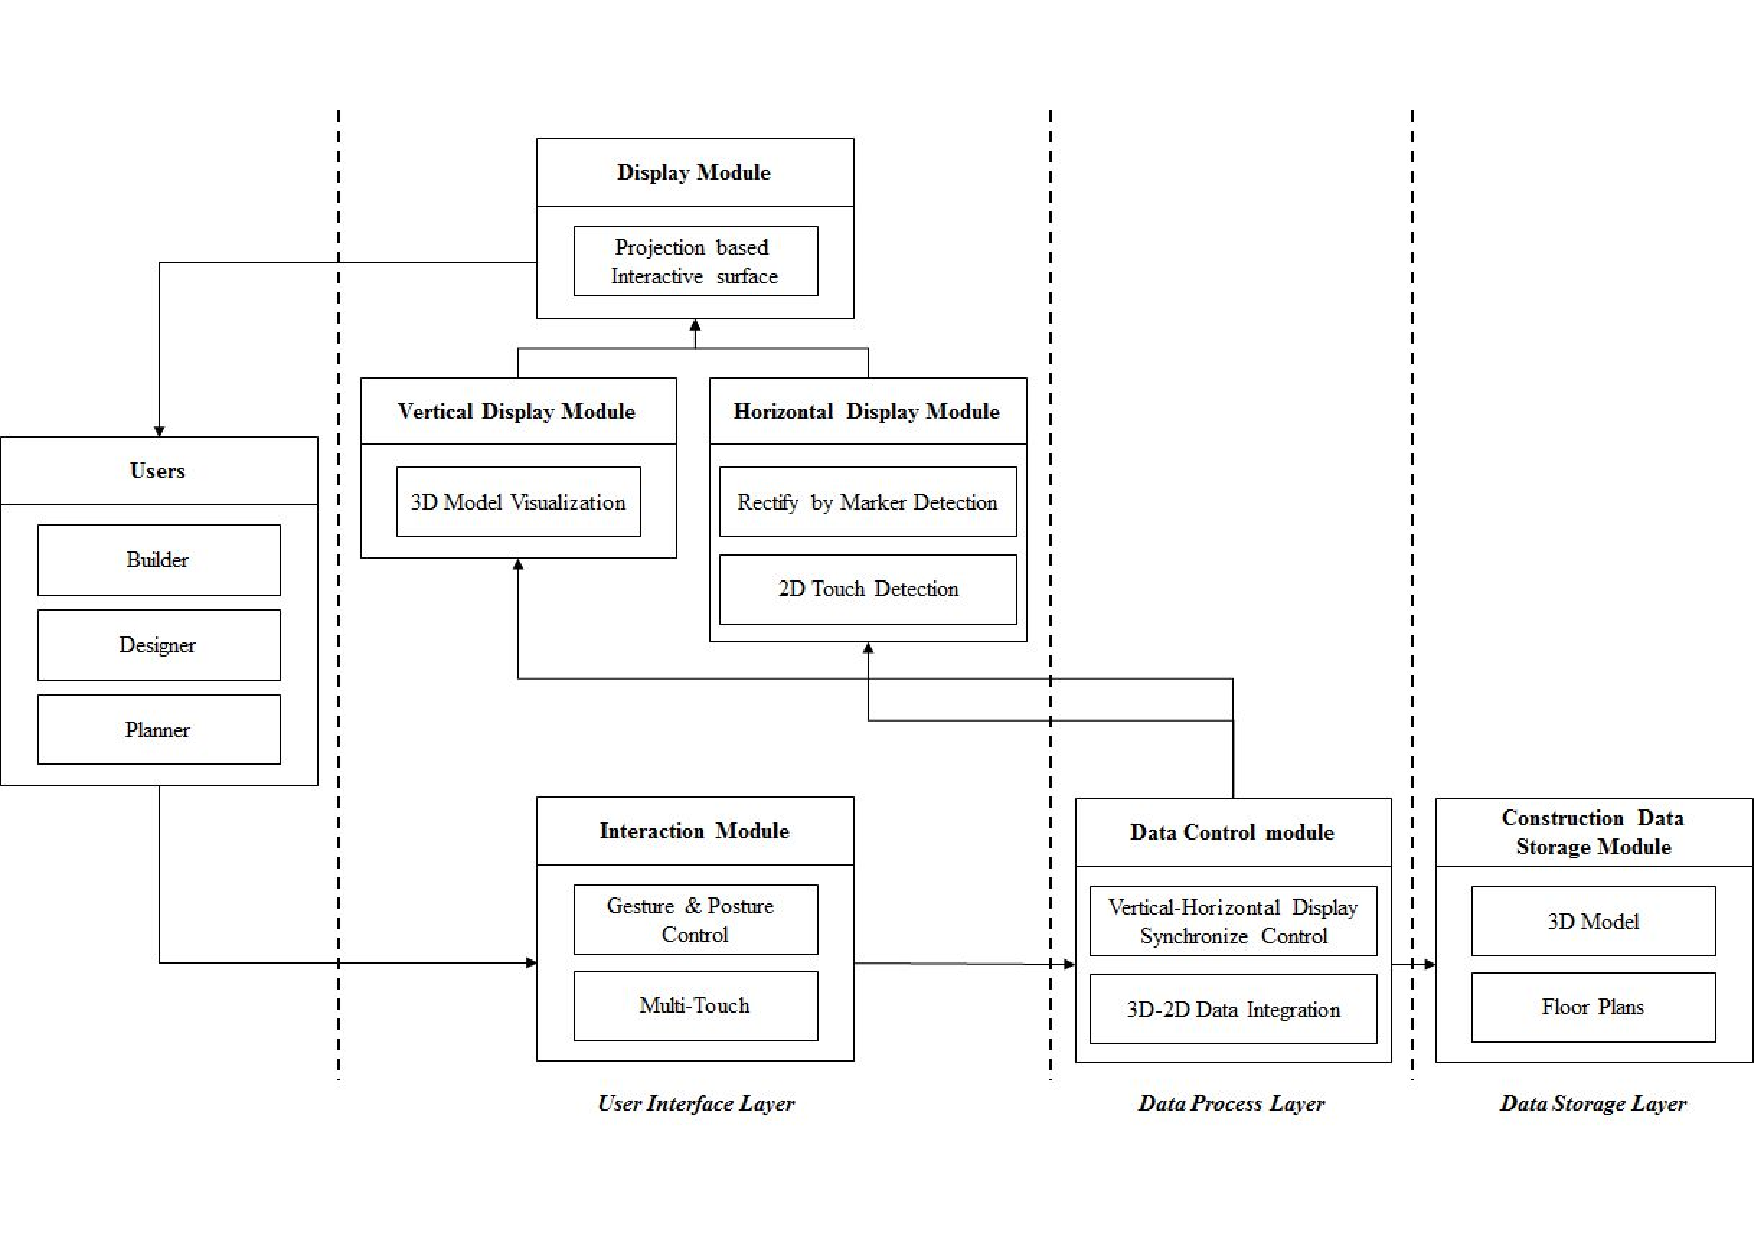
\includegraphics[width=\textwidth]{3-System/architecture_}
	\caption{The system architecture of proposed system}
    \label{fig:architecture}
\end{figure}

본 논문에서는 현장에서 필요한 정보를 이해하기 쉬운 형태로 제공하고, 현장 작업자들의 협업 지원을 위해 Projection 기반 시스템을 이용하여 시스템을 구성하였다.  Projection 기반인 Interactive Surface는 Vertical/Horizontal Display로 구성되며, 이를 이용하여 2D Floor Plan 과 3D 건축 모델의 정보를 제공한다. 또한 상호작용을 위해 제스처, 터치 기능을 지원함으로써 직관적인 제어가 가능하도록 하였다. 
그림 \ref{fig:architecture}에서 보듯이 시스템은 User Interface Layer, Data Process, Data Storage Layer 등 총 3개의 Layer로 구성되어 있다. 

\begin{itemize}
\item User Interface Layer : Vertical/Horizontal Display를 제스처, 터치 기능을 이용하여 직접적으로 제어 하며, 실시간 모델에 대한 상태 확인이 가능
\item Data Process Layer : 사용자가 입력한 건축 모델에 대한 제어를 인식하고, 결과를 Vertical/Horizontal Display에 실시간 반영하는 역할을 수행
\item Data storage Layer : 3D Model, Floor Plane와 같은 건축 정보 관리
\end{itemize}

%%%%%%%%%%%%%%%%%%%%%%%%%%%%%%%%%%%%%%%%%%%%%%%%%%%%%%%%%%%%%%%%%%%%%%%
\subsection{System Overview}
\begin{figure}[ht!]
	\centering
    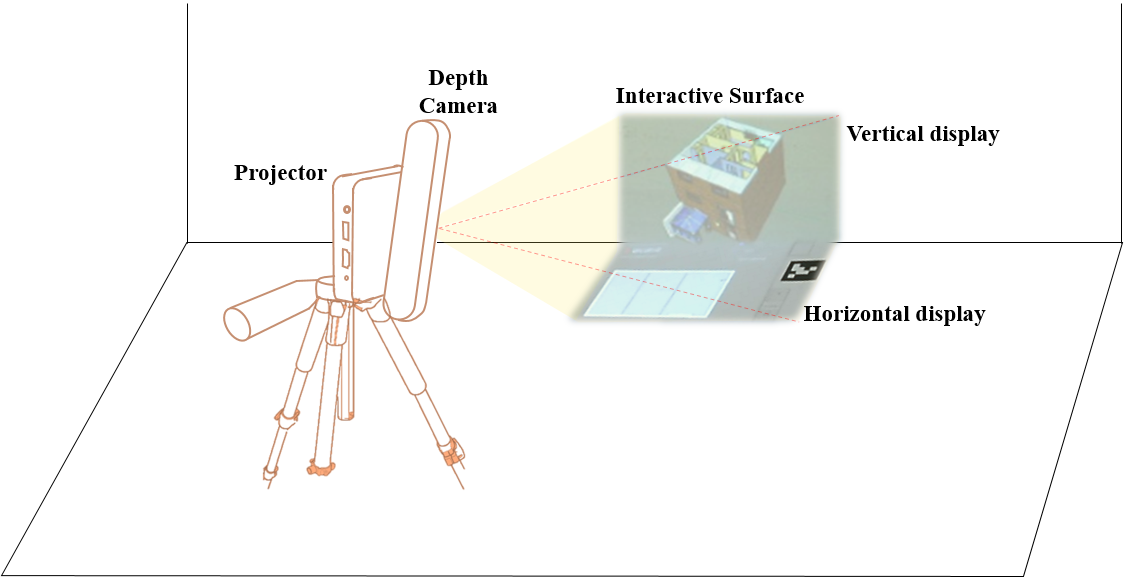
\includegraphics[width=\textwidth]{3-System/overview}
	\caption{System Components}
    \label{fig:overview}
\end{figure}

제안하는 시스템의 구조는 그림 \ref{fig:overview} 과 같다. 컬러 영상을 이용하여 도면에 위치한 마커를 인식하여 전체 프로젝션 위치를 추정한다. Horizontal display에서는 도면위에 2D 정보를 프로젝션 하며, Vertical display는 도면에 맞는 3D 모델을 출력한다. 두 개의 Display는 서로 동기화 되며 동작하며, 사용자는 직관적인 제스처 및 터치 상호작용을 통해 컨텐츠 제어가 가능하다.  

%%%%%%%%%%%%%%%%%%%%%%%%%%%%%%%%%%%%%%%%%%%%%%%%%%%%%%%%%%%%%%%%%%%%%%%
\subsection{System Implementation}
\subsubsection{System Hardware}
\begin{figure}[ht!]
	\centering
    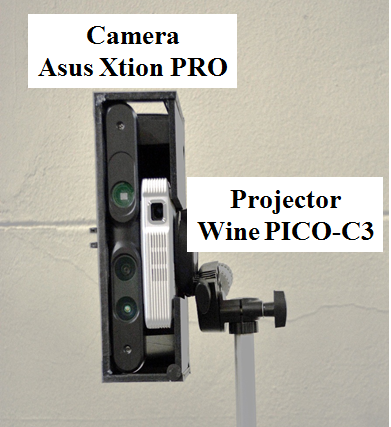
\includegraphics[width=0.4\textwidth]{3-System/hardware}
	\caption{Hardware Configuration}
    \label{fig:hardware}
\end{figure}
3D Interactive Surface의 구성을 위해 그림 \ref{fig:hardware}과 같이 Projection 기반의 하드웨어를 구성하였다. 본 연구에서 사용된 카메라는 Asus Xtion PRO, 프로젝터는 Wine PICO-C3를 사용하였으나, 다른 기종의 하드웨어를 사용하여도 무방하다. 카메라는 Horizontal Display 의 마커를 인식하고 사용자의 제스처와 터치를 인식하는데 사용되며, 프로젝터를 이용하여 영상을 출력한다. 인식하는데 카메라와 프로젝터는 캘리브레이션을 위해 서로 고정된 형태로 구성되어 있다. 이를 이용하여 마커를 인식하고, L-shape 벽면에 프로젝션 함으로써, 한 대의 프로젝터를 이용하여 Vertical/Horizontal Display 출력 및 제어가 가능하다.

\subsubsection{Portable Multiscreen System}
본 논문에서는 2차원 데이터와 3차원 모델을 동시에 제공하기 위하여 Multiscreen interactive screen 기술을 이용하였다. 기존의 multiscreen interactive screen 기술들은 사전에 두 interactive surface 의 위치관계를 calibration하여 제공하기 때문에 Stationary한 한계가 있다. 하지만 본 논문에서는 건축 현장에서의 활용을 위하여 Image Marker를 이용하여 portable한 환경에서 실시간 calibration 기술을 개발하였다. Calibration 과정은 카메라-프로젝션 간의 영상 캘리브레이션, 프로젝션과 각 Display간의 위치 캘리브레이션으로 나눌 수 있다. 
먼저, 카메라와 프로젝터는 위치가 고정되어 사용되기 때문에 사전에 calibration을 수행할 수 있다. 이 단계에서는 그림 \ref{fig:procam_calibration}과 같은 calibration board를 활용하여 수행되었다.
\begin{figure}[ht!]
	\centering
    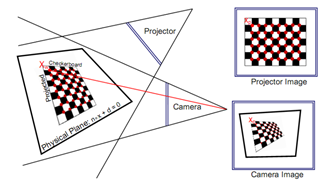
\includegraphics[width=0.4\textwidth]{3-System/calibration1}
	\caption{Projector-Camera Calibration}
    \label{fig:procam_calibration}
\end{figure}

이 후 그림 \ref{fig:multiscreen_calibration}와 같이 Horizontal screen과 vertical screen 간의 multiscreen calibration은 마커를 이용하여 위치를 추정하였다. 
% \begin{figure*}[!ht]
\begin{figure*}[!ht]
	\centering
        \begin{subfigure}[b]{0.8\textwidth}
            \centering
           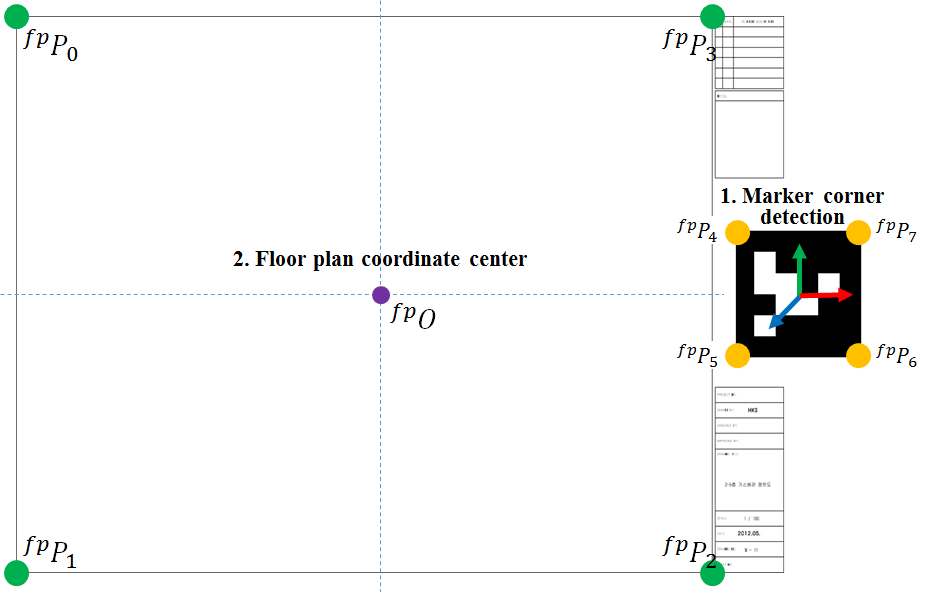
\includegraphics[width=\textwidth]{3-System/marker_calibration1}
                \caption{}
                \label{fig:marker_1}
        \end{subfigure}
        \\
        \begin{subfigure}[b]{0.8\textwidth}
	        \centering
              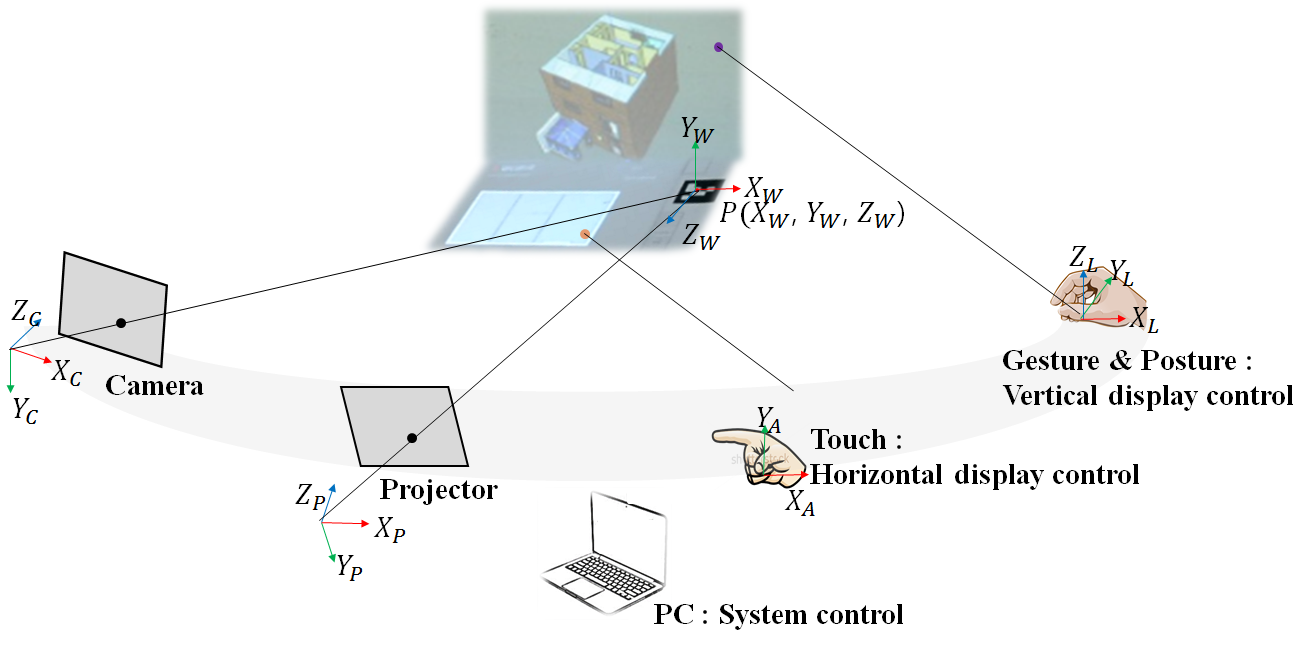
\includegraphics[width=\columnwidth]{3-System/marker_calibration2}
              \caption{}
              \label{fig:hardware}
        \end{subfigure}%
	\caption{Multiscreen Calibration}
    \label{fig:multiscreen_calibration}
\end{figure*}

\textcolor{red}{Horizontal-Vertical Screen Calibration 관련 수식 추가}

위에서 설명한 캘리브레이션을 수행하게 되면 프로젝션을 위한 Vertical/Horizontal Display에 대한 위치가 결정 된다. 이러한 시스템을 이용하여 실시간 위치 추정이 가능하며, Portable 환경에서 한 대의 프로젝터를 이용하여 Multi-view를 생성하는 것을 가능하게 한다. 그림 \ref{fig:marker_calibration}은 실제 캘리브레이션을 수행하고, 마커를 이용하여 Vertical/Horizontal Display의 위치를 추정하는 단계이다. 
\begin{figure}[ht!]
	\centering
    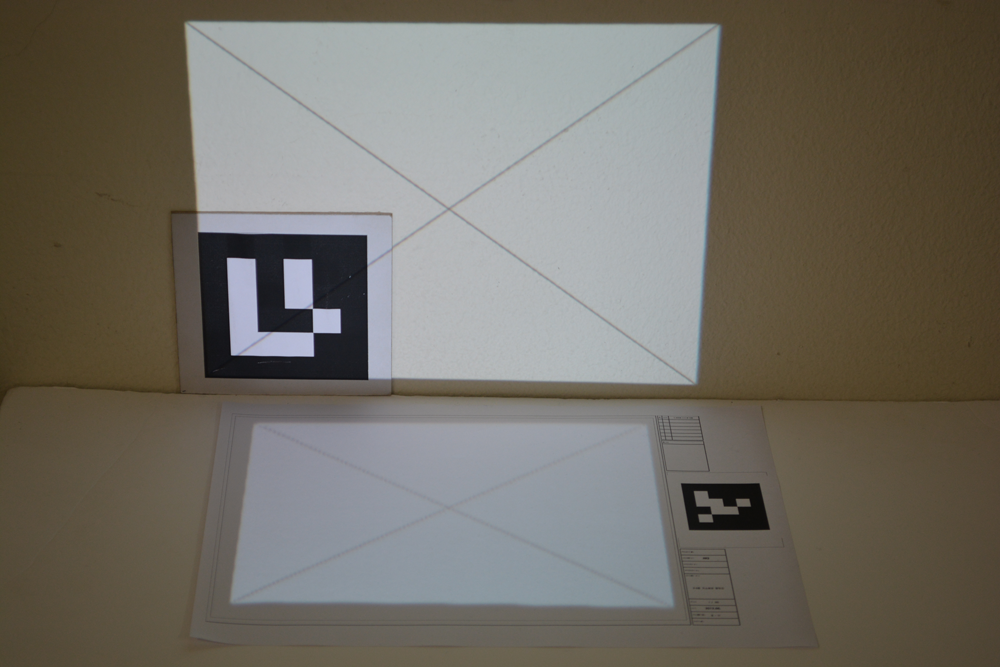
\includegraphics[width=\textwidth]{3-System/rectified}
	\caption{Marker-based Calibration}
    \label{fig:marker_calibration}
\end{figure}
입력된 영상을 기반으로 Vertical/Horizontal Display에 설정에 대한 전체적인 Flowchart는 다음과 같다. 
\textcolor{red}{Calibration Flowchart 삽입}

%%%%%%%%%%%%%%%%
\subsubsection{Interaction Implementation}
건축 현장에서 별도의 인터페이스 없이 상호작용을 제공하기 위하여 터치와 in-air 제스처 인식 기술을 제공한다.
\textcolor{red}{세부 내용 작성}



%%%%%%%%%%%%%%%%
\subsection{Interaction Design}

제안하는 연구는 프로젝션 화면을 이용하여 건축현장에서 협업을 지원하고, 정보공유를 원활 하게 한다. 또한 제공된 컨텐츠를 제어 및 수정하기 위해 다양한 상호작용 방법을 지원한다. 
\subsubsection{3D Model Manipulation}
설계도는 3차원 모델의 구조, 형상, 치수 등을 일정한 규약에 따라 2차원으로 투영하여 표현한 것이다. 제안하는 시스템은 2차원 설계도를 이용하여 3차원 모델의 정보를 현장에서 바로 확인할 수 있으며 제어 가능하다. 이를 위해 3차원 공간에서 손을 인식하는 NUI 기술을 통해 3차원 모델을 제어하고자 한다.
\begin{figure*}[!ht]
	\centering
        \begin{subfigure}[b]{0.32\textwidth}
	        \centering
                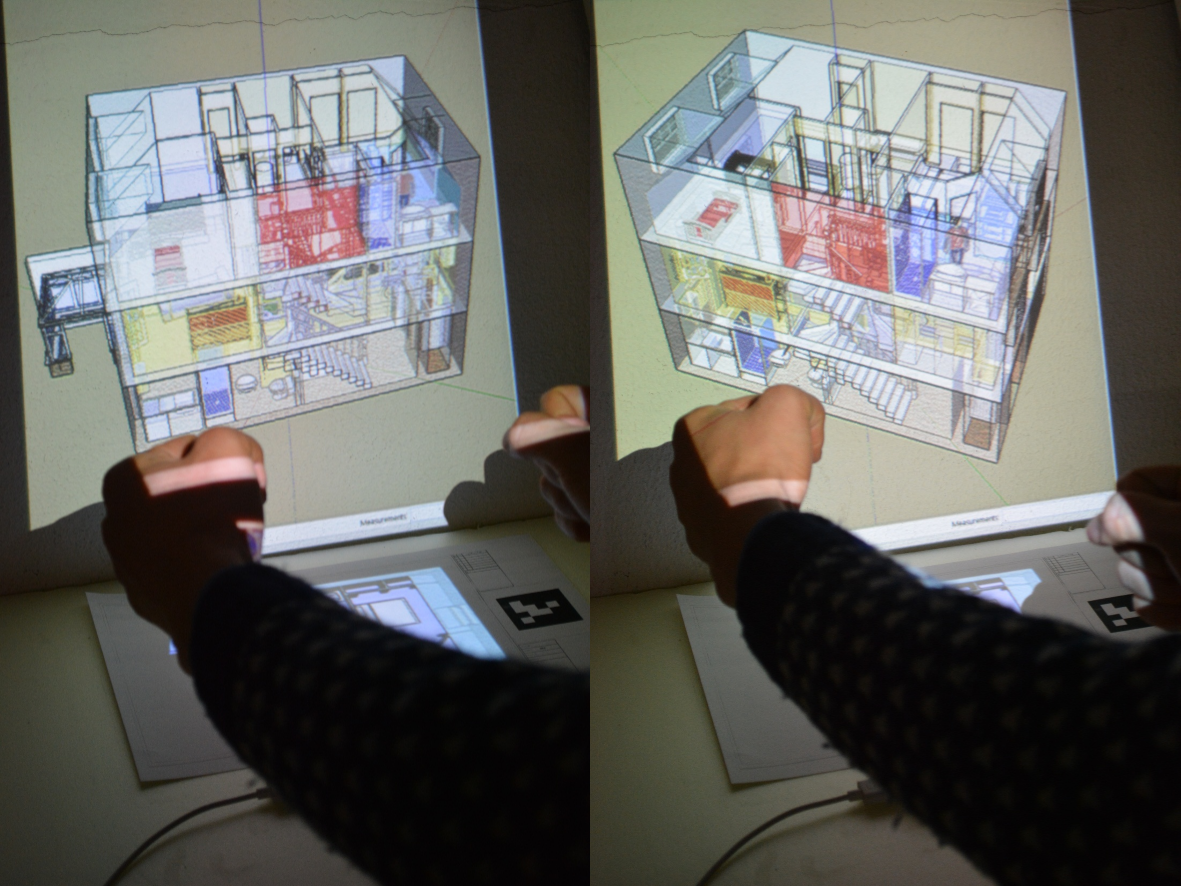
\includegraphics[width=\textwidth]{4-Interaction_Design/3d_rotate}
                \caption{Rotating the Model}
                \label{fig:rotate}
        \end{subfigure}%
        \hfill
        \begin{subfigure}[b]{0.32\textwidth}
            \centering
            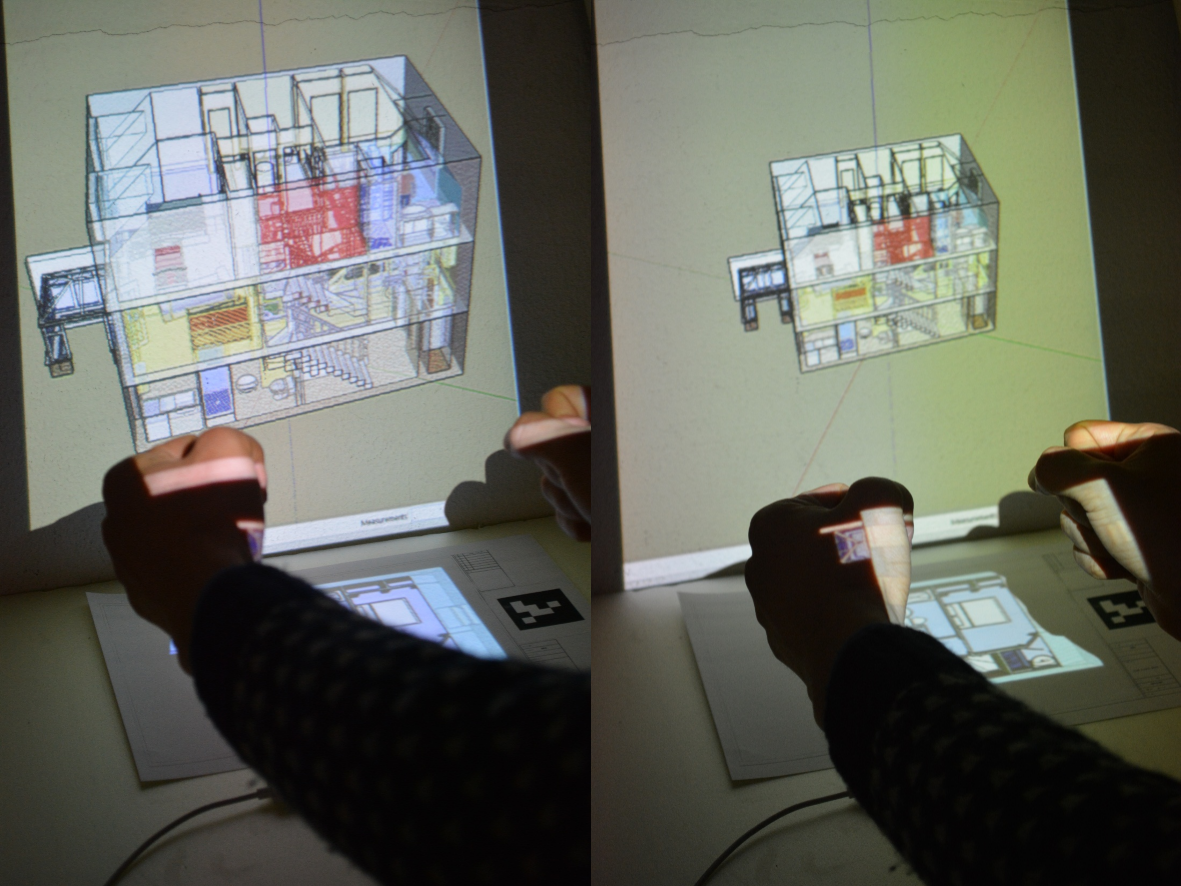
\includegraphics[width=\textwidth]{4-Interaction_Design/3d_scale_two_hand}
                \caption{Scaling by Two Hand Gesture}
                \label{fig:scale_two_hand}
        \end{subfigure}
        \hfill
        \begin{subfigure}[b]{0.32\textwidth}
            \centering
            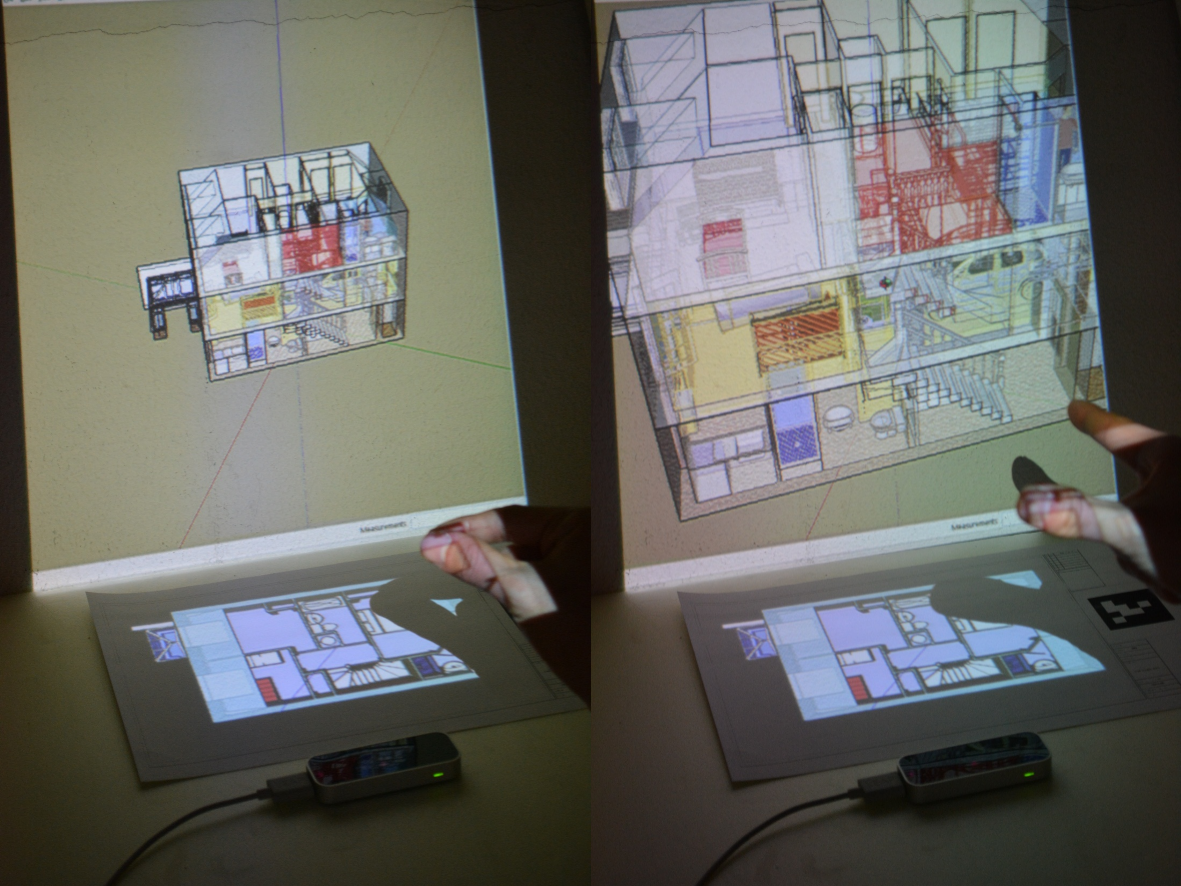
\includegraphics[width=\textwidth]{4-Interaction_Design/3d_scale_one_hand}
                \caption{Scaling by One Hand Gesture}
                \label{fig:scale_pinch}
        \end{subfigure}
	\caption{3D Manipulation}
    \label{fig:3d_mani}
\end{figure*}

사용자의 손 또는 손가락을 인식하여 3D 건축 모델의 회전 기능을 가능하게 한다. 그림 \ref{fig:rotate}처럼 사용자의 양손을 위치를 기준으로 3차원 공간에서 회전을 수행한다. 
Rotating 기능뿐만 아니라, 3D 모델을 확대하거나 축소하여 보는 Scaling 기능을 제공한다. 이 때, 직관적인 상호작용을 위하여 두 가지 모드의 Scaling 방법을 제공한다. 첫 번째 방법은, Rotating 기능과 동시에 수행할 수 있도록 양 손을 이용한 Scaling 기능을 수행 한다. 이는 그림 \ref{fig:scale_two_hand}과 같이 양손을 인식하고 거리 변화를 측정하여 3D 모델의 크기 조절을 가능하게 한다. 두 번째 방법은 그림 \ref{fig:scale_pinch}과 같이 손의 엄지와 검지 손가락을 이용하여 핀치 제스처를 인식하고 핀치 제스처의 움직임을 기반으로 3D 모델의 크기 조절이 가능하게 한다.

\subsubsection{Querying Specific Floor Plan}
특정 평면도의 정보에 접근할 필요가 있을 때, 그림 \ref{fig:layer}과 같이 손가락을 인식하여 평면도의 정보를 선택하여 확인 가능 하다. 시스템과 건축 모델링툴(ex, SketchUp)을 동기화하여 건물의 도면 정보를 이용하여 전체 건물 정보에서 특정 평면의 정보를 Horizontal Display에 증강 하도록 한다. 
 \begin{figure}[h!]
\centering
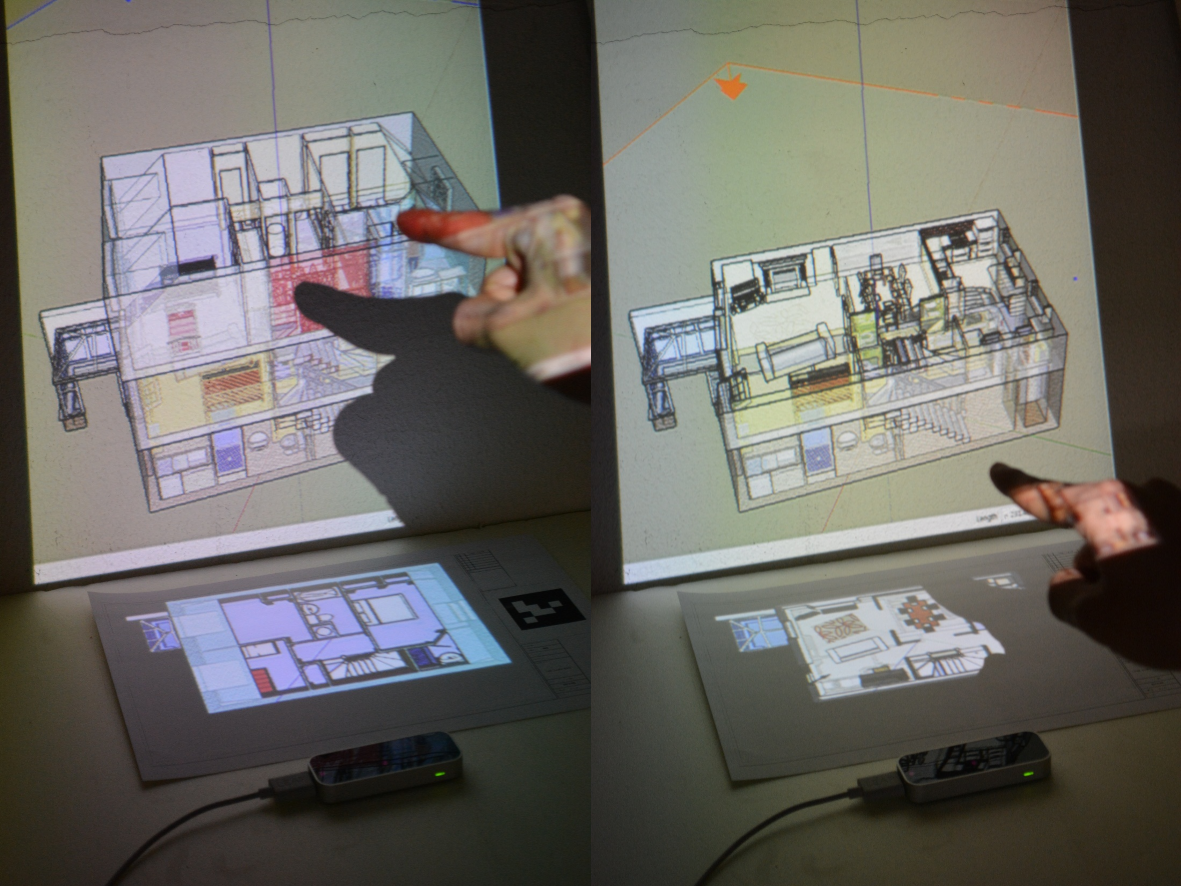
\includegraphics[width=0.4\textwidth]{4-Interaction_Design/query_plane}
\caption{Querying Specific Floor Plan}
\label{fig:layer}
\end{figure}


\subsubsection{Additional Information Retrieval}

또한, 취득한 도면의 부가적인 정보를 이용하여 면적이나 부피 등을 파악해야 하는 경우도 발생한다. 예를 들어 \cite{song_penlight:_2009}에서 제안한 것과 같이 건축 도면에서 부가적인 Dimension 정보를 제공하는 것은 현장에서 유용하게 사용될 수 있다. 본 연구에서는 건축 모델링툴 중 SketchUp에서 제공하는 Entity 정보를 이용하여 평면의 면적, 부피 등의 정보를 사용자에게 제공하였다. 또한 3D 정보를 제공함으로써 in-air 터치한 벽면의 넓이나 기둥의 높이 등의 3차원 Entity 정보를 제공할 수 있다. 
\begin{figure*}[!ht]
	\centering
        \begin{subfigure}[b]{0.55\textwidth}
	        \centering
                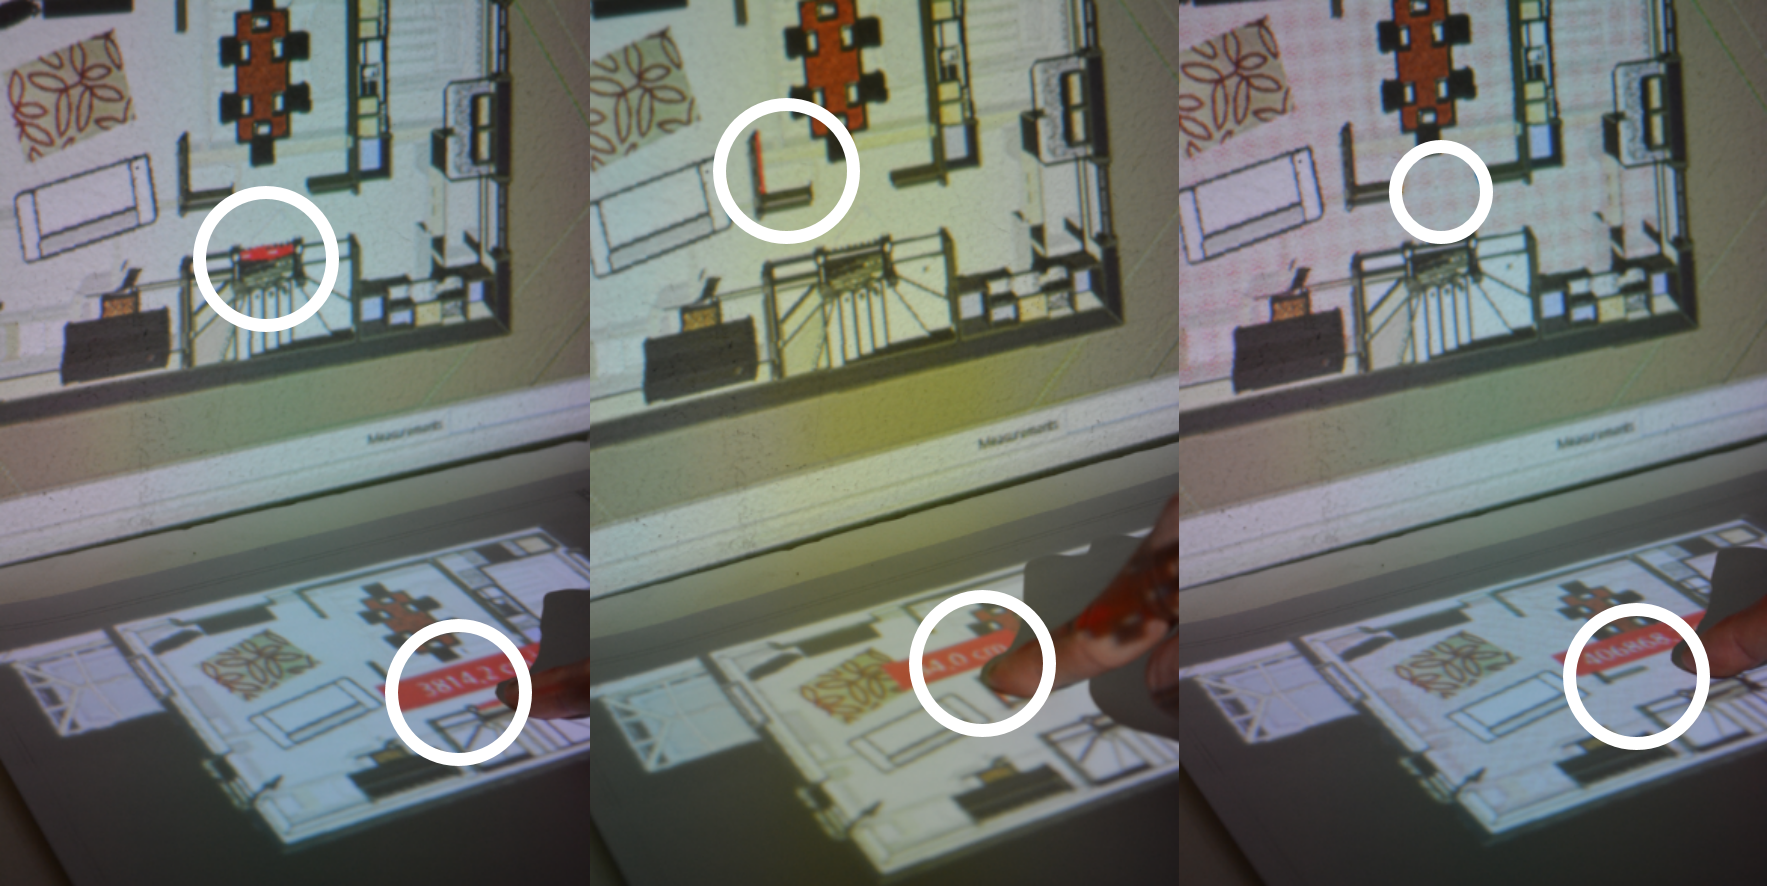
\includegraphics[width=\textwidth]{4-Interaction_Design/2d_info}
                \caption{Querying 2D information - length, area, volumn of specific entity}
                \label{fig:2d_info}
        \end{subfigure}%
        \hfill
        \begin{subfigure}[b]{0.37\textwidth}
            \centering
            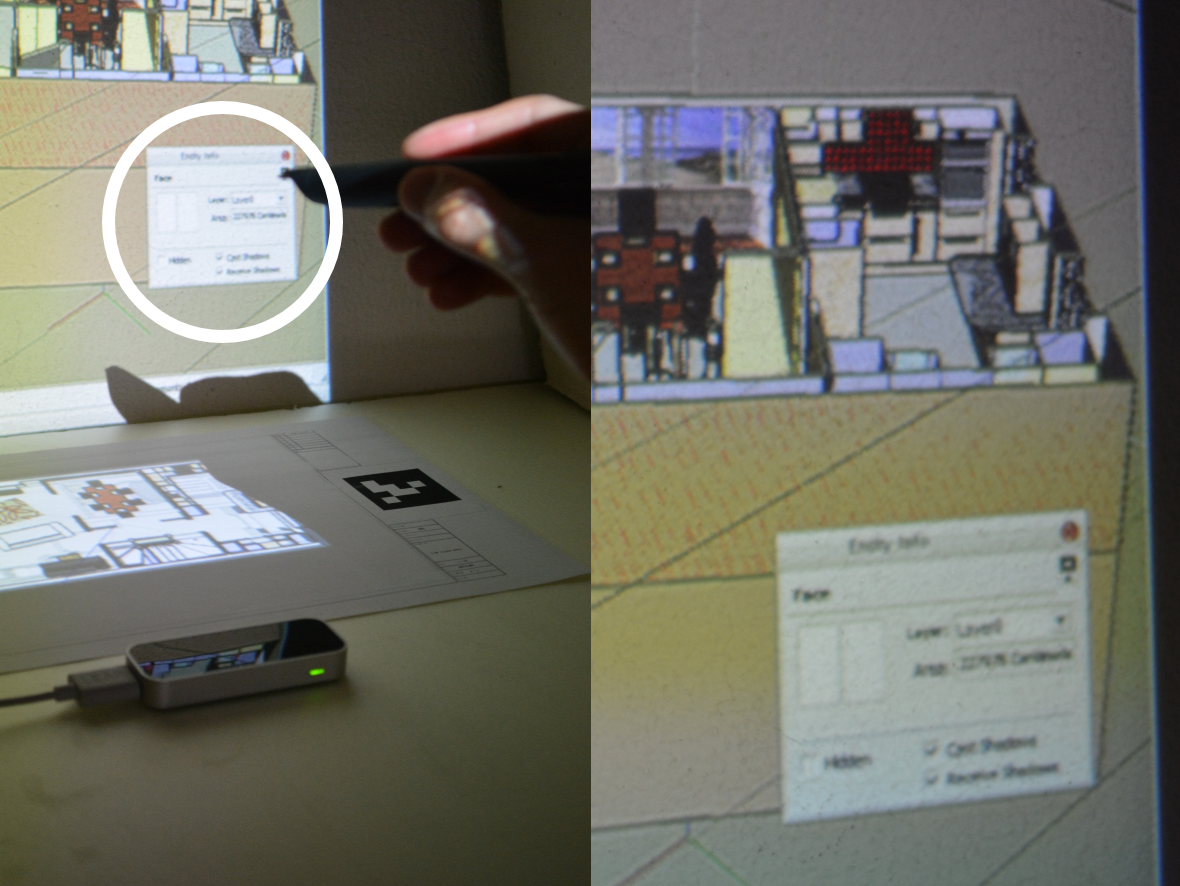
\includegraphics[width=\textwidth]{4-Interaction_Design/3d_info}
                \caption{3D information}
                \label{fig:3d_info}
        \end{subfigure}
	\caption{3D Manipulation}
    \label{fig:infor}
\end{figure*}


2D Information Retrieval
2D 정보 제공은 그림 \ref{fig:2d_info}와 같이 도면에 나타난 벽면의 길이나 바닥 면, 가구 등의 부피 등의 도면을 직접 터치함으로써 획득할 수 있다. 이는 해당 건축 도면 상에서 터치된 2차원 위치를 이용하여 시스템상의 Entity 정보를 이용하여 획득 가능하다.
3D Information Retrieval
3D 정보 제공은 그림 \ref{fig:3d_info}와 같이 제스처를 이용하여 3D 모델을 선택함으로써 정보를 제공받게 된다. 2D에 대한 정보 획득이 도면을 이용한 Horizontal Display를 이용한 입력이었다면, 3D에 대한 정보는 Vertical Display를 직접적으로 터치함으로써 입력이 제공된다. 

\subsubsection{On-site Editing}
현 시스템에서 도면의 변경이 필요한 경우, 정보에 대한 접근과 수정이 어렵기 때문에 변경사항을 실시간으로 반영하기 어렵다. 본 연구에서는 사용자의 손 움직임과 터치를 이용하여 건축 모델을 실시간 선택하고, 이동하거나 수정 가능하도록 하였다. 
\begin{figure}[h!]
    \centering
        \begin{subfigure}[b]{0.49\columnwidth}
            \centering
                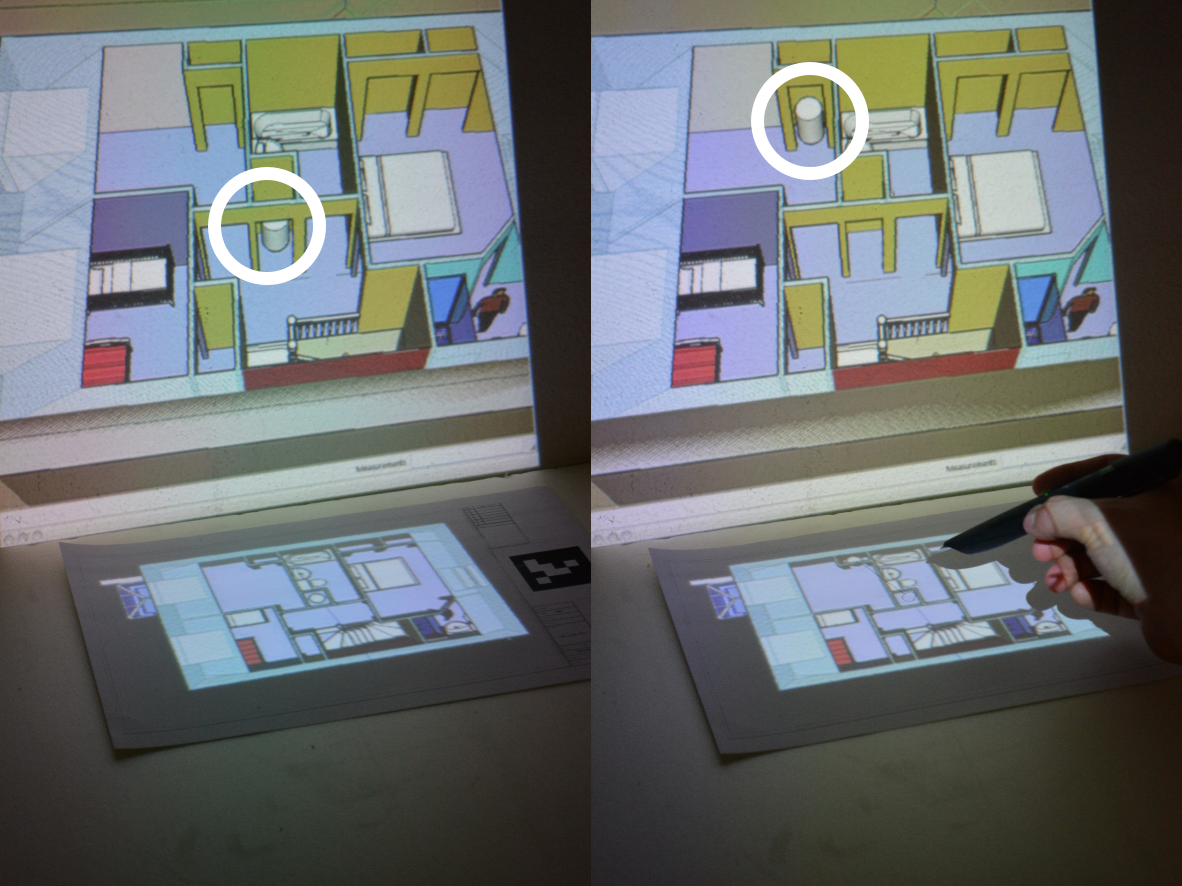
\includegraphics[width=1.0\columnwidth, height=3.6cm]{4-Interaction_Design/2d_move}
                \caption{Modifying 2D Entity using Pen}
                \label{fig:Pen_move}
        \end{subfigure}%
        \hfill
        \begin{subfigure}[b]{0.49\columnwidth}
            \centering
            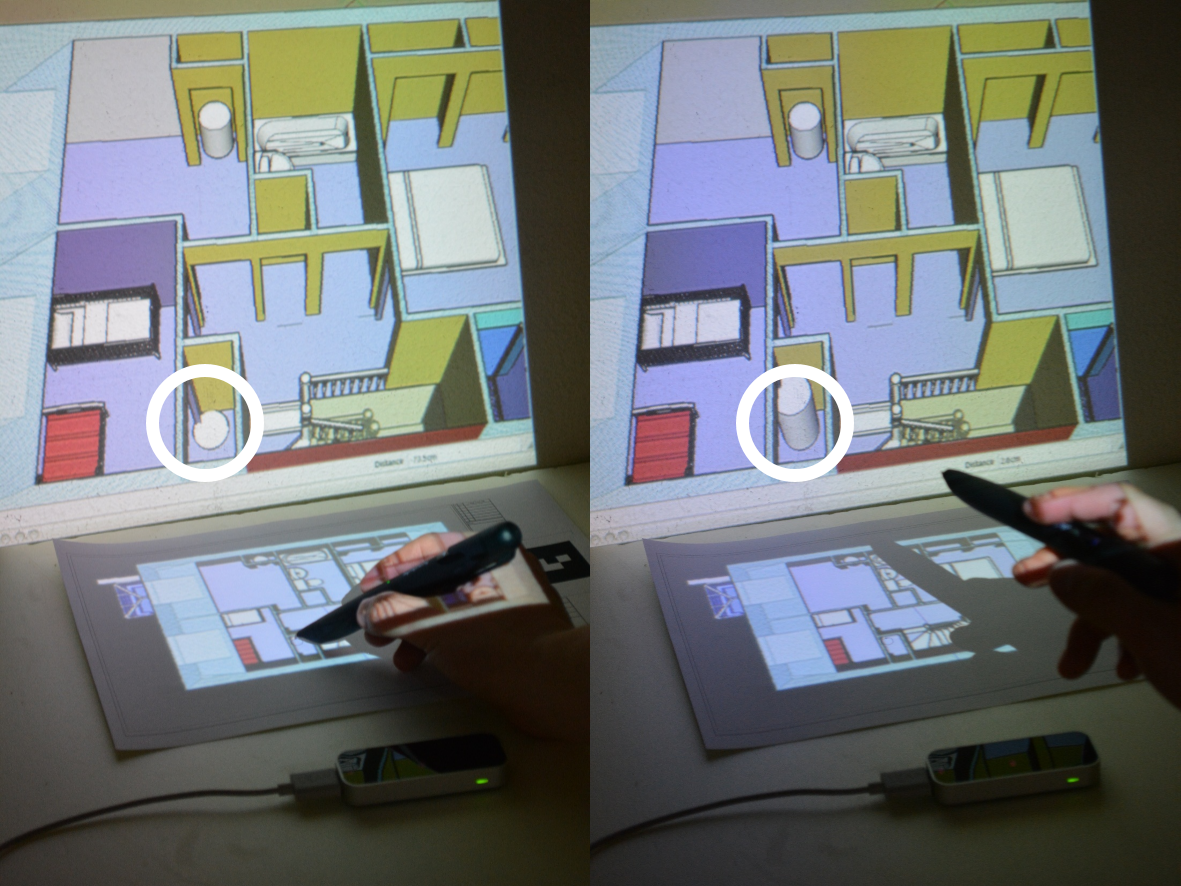
\includegraphics[width=1.0\columnwidth, height=3.6cm]{4-Interaction_Design/3d_note}
                \caption{Modifying 3D Entity in-air}
                \label{fig:Annotation}
        \end{subfigure}
    \caption{On-site Editing using Pen}
    \label{fig:edit}
\end{figure}

\textcolor{red}{제공된 컨텐츠를 정리하고, 전체적인 그림으로 표현, 삽입 예정}
